% Options for packages loaded elsewhere
\PassOptionsToPackage{unicode}{hyperref}
\PassOptionsToPackage{hyphens}{url}
%
\documentclass[
  12pt,
]{article}
\usepackage{amsmath,amssymb}
\usepackage{iftex}
\ifPDFTeX
  \usepackage[T1]{fontenc}
  \usepackage[utf8]{inputenc}
  \usepackage{textcomp} % provide euro and other symbols
\else % if luatex or xetex
  \usepackage{unicode-math} % this also loads fontspec
  \defaultfontfeatures{Scale=MatchLowercase}
  \defaultfontfeatures[\rmfamily]{Ligatures=TeX,Scale=1}
\fi
\usepackage{lmodern}
\ifPDFTeX\else
  % xetex/luatex font selection
  \setmainfont[]{Times New Roman}
\fi
% Use upquote if available, for straight quotes in verbatim environments
\IfFileExists{upquote.sty}{\usepackage{upquote}}{}
\IfFileExists{microtype.sty}{% use microtype if available
  \usepackage[]{microtype}
  \UseMicrotypeSet[protrusion]{basicmath} % disable protrusion for tt fonts
}{}
\makeatletter
\@ifundefined{KOMAClassName}{% if non-KOMA class
  \IfFileExists{parskip.sty}{%
    \usepackage{parskip}
  }{% else
    \setlength{\parindent}{0pt}
    \setlength{\parskip}{6pt plus 2pt minus 1pt}}
}{% if KOMA class
  \KOMAoptions{parskip=half}}
\makeatother
\usepackage{xcolor}
\usepackage[left=2.54cm,right=2.54cm,top=2.54cm,bottom=2.54cm]{geometry}
\usepackage{graphicx}
\makeatletter
\def\maxwidth{\ifdim\Gin@nat@width>\linewidth\linewidth\else\Gin@nat@width\fi}
\def\maxheight{\ifdim\Gin@nat@height>\textheight\textheight\else\Gin@nat@height\fi}
\makeatother
% Scale images if necessary, so that they will not overflow the page
% margins by default, and it is still possible to overwrite the defaults
% using explicit options in \includegraphics[width, height, ...]{}
\setkeys{Gin}{width=\maxwidth,height=\maxheight,keepaspectratio}
% Set default figure placement to htbp
\makeatletter
\def\fps@figure{htbp}
\makeatother
\setlength{\emergencystretch}{3em} % prevent overfull lines
\providecommand{\tightlist}{%
  \setlength{\itemsep}{0pt}\setlength{\parskip}{0pt}}
\setcounter{secnumdepth}{5}
\ifLuaTeX
  \usepackage{selnolig}  % disable illegal ligatures
\fi
\IfFileExists{bookmark.sty}{\usepackage{bookmark}}{\usepackage{hyperref}}
\IfFileExists{xurl.sty}{\usepackage{xurl}}{} % add URL line breaks if available
\urlstyle{same}
\hypersetup{
  hidelinks,
  pdfcreator={LaTeX via pandoc}}

\author{}
\date{\vspace{-2.5em}}

\begin{document}

\hypertarget{declaration}{%
\subsubsection{Declaration}\label{declaration}}

We declare that the following project is evidence of our own work that
has not been submitted previously for academic credit. All group
members, who have all actively contributed, submit this assignment as an
original piece of work.

\begin{itemize}
\tightlist
\item
  Conceptualisation, X.X. and Y.Y.;
\item
  Methodology, X.X.;
\item
  Software, X.X.;
\item
  Validation, X.X., Y.Y. and Z.Z.;
\item
  Formal Analysis, X.X.;
\item
  Investigation, X.X.;
\item
  Resources, X.X.;
\item
  Data Curation, X.X.;
\item
  Writing -- Original Draft Preparation, X.X.;
\item
  Writing -- Review \& Editing, X.X.;
\item
  Visualisation, X.X.
\end{itemize}

\hypertarget{abstract}{%
\subsubsection{Abstract}\label{abstract}}

This project conducts a comprehensive exploratory data analysis (EDA) of
the ``Stack Overflow Annual Developer Survey 2023,'' collecting
responses from more than 90,000 developers worldwide. The main aim is to
investigate the factors affecting the compensation of developers using
various selected determinants.

Our analysis demonstrates important information about developer
compensation by exploring the impact of experience, education level, and
technological expertise. In conducting our analysis, we used regression
models, leveraging the survey's detailed classification and clustering
information to calculate the standard errors of the survey estimates
accurately. We used graphs to evaluate the relationships between various
categorical variables. We detailed our findings and conducted hypothesis
testing to evaluate the relationships. Additionally, we addressed
nonresponse issues by using multiple imputation techniques to address
missing data and ensure robustness in our findings.

This analysis provides insight into compensation dynamics among
developers worldwide by addressing critical factors affecting yearly
compensation.

\hypertarget{contents}{%
\subsubsection{Contents}\label{contents}}

\begin{enumerate}
\def\labelenumi{\arabic{enumi}.}
\tightlist
\item
  \textbf{Declaration}
\item
  \textbf{Abstract}
\item
  \textbf{Introduction}

  \begin{itemize}
  \tightlist
  \item
    Project Rationale
  \item
    Aim
  \end{itemize}
\item
  \textbf{Data Description}
\item
  \textbf{Survey Methodology}

  \begin{itemize}
  \tightlist
  \item
    Key Principles

    \begin{itemize}
    \tightlist
    \item
      Scope and Scale
    \item
      Duration and Timing
    \end{itemize}
  \item
    Survey Design
  \item
    Evaluation of Methodologies

    \begin{itemize}
    \tightlist
    \item
      Recruitment Methods
    \item
      Geography
    \item
      Adaptive Questionnaire
    \item
      Handling of Compensation Data
    \item
      Technological Inclusion
    \item
      Randomisation of Questions
    \item
      Data Analysis Adjustments
    \item
      Survey Language
    \end{itemize}
  \item
    Non-Response
  \end{itemize}
\item
  \textbf{Data Analysis}

  \begin{itemize}
  \tightlist
  \item
    Data Description
  \item
    Exploratory Data Analysis (EDA)
  \item
    Data Cleaning and Manipulation
  \item
    Feature Selection and Data Curation
  \end{itemize}
\item
  \textbf{Implementation}
\item
  \textbf{Results}

  \begin{itemize}
  \tightlist
  \item
    Numerical Response
  \item
    Categorical Response
  \item
    Regression Analysis
  \end{itemize}
\item
  \textbf{Discussion}

  \begin{itemize}
  \tightlist
  \item
    Successes
  \item
    Limitations
  \end{itemize}
\item
  \textbf{Conclusion}
\item
  \textbf{References}
\item
  \textbf{Appendix}
\end{enumerate}

\hypertarget{introduction}{%
\subsubsection{Introduction}\label{introduction}}

The Stack Overflow Annual Developer Survey 2023 is a comprehensive
survey that gathers valuable insights from a large and diverse
population of software developers worldwide. The survey covers a wide
array of topics, including developer roles, programming languages,
tools, frameworks, job satisfaction, career aspirations, demographic
characteristics and salaries. With a focus on capturing the evolving
developer experience and understanding the impact of emerging
technologies like AI/ML on developers' workflows, the survey offers a
unique opportunity to investigate the determinants of developer
compensation on a global scale.

\hypertarget{project-rationale}{%
\paragraph{Project Rationale}\label{project-rationale}}

The tech industry is characterised by rapid advancements and constant
change, making it imperative to understand the determinants of developer
compensation. The factors that influence compensation have far-reaching
implications, not only for individual developers' career trajectories
but also for the overall productivity and innovation within
organisations. It is therefore vital to study the interplay between the
aforementioned factors in determining compensation.

\hypertarget{aim}{%
\paragraph{Aim}\label{aim}}

The primary objective of this project is to conduct a detailed
exploratory data analysis (EDA) of the Stack Overflow Annual Developer
Survey 2023, focusing on understanding the factors that affect developer
compensation across the world. We aim to use `compensation' as the
continuous response variable in our regression models to predict
compensation based on various predictors such as organisation size,
education level, work experience, and role in the industry (developer
type). By analysing these, we plan to discover insights into the career
paths of developers and the evolving technology landscape, providing
valuable information for stakeholders in the tech industry. This
analysis will highlight potential fields for the developer community and
identify which variables are more influential.

\hypertarget{data-description}{%
\subsubsection{Data Description}\label{data-description}}

By collecting the voice of developers, the Stack Overflow Annual
Developer Survey 2023 enables analysts, IT leaders, reporters and other
developers to stay up to date with the latest trends and technologies
that are shaping the industry. The extensive reach and depth of
information provided by the survey not only helps provides context in
understanding where trends in technology are heading, but also offers
key attributes that can potentially influence developer compensation.
Through a thorough analysis of this rich dataset, we can gain a deeper
understanding of the complex interplay between various variables, such
as developer roles, skills, experience, and geographic location, that
contribute to determining remuneration in the global tech industry.

The rows within this data set are representative of each respondent who
filled out the survey and each column is representative of each question
within the survey. As previously identified, there is a large number of
missing values as respondents were unable to answer questions based on
inability or branching of questions.

\hypertarget{survey-methodology}{%
\subsubsection{Survey Methodology}\label{survey-methodology}}

\newline
\newline

\hypertarget{key-principles}{%
\paragraph{Key Principles}\label{key-principles}}

\newline
\newline

\textbf{Scope and Scale}: The survey reached 89,184 qualified software
developers from 185 countries, indicating a broad global representation.
The qualification for analysis was based on respondents' consenting to
share their data and the completion of all required questions.
Approximately 2,000 responses were excluded due to incomplete data.
\newline \newline

\textbf{Duration and Timing}: The survey was conducted from May 82023,
to May 19, 2023. The median response time was nearly 18 minutes, which
increased from the previous year due to the inclusion of additional
questions. \newline \newline \newline

\hypertarget{survey-design}{%
\paragraph{Survey Design}\label{survey-design}}

The objective of this survey was to obtain data on a wide range of
topics to help infer and provide insights into trends and technology
that are shaping the developers industry. The survey contained questions
relating to the objective details on the respondents, such as, the years
they've spent coding, their salary and their profession. This was
combined with questions designed to elicit more subjective responses in
relation to the technology landscape, such as, their thoughts on the
usefulness of AI to their work and whether Stack Overflow has been
helpful. \newline

The questionnaire contained a mix of questions in the form of
single-response multiple choice, multiple-response multiple choice and
short answers that resulted in responses of categorical or numerical
natures. Some multiple choice questions themselves contained response
options that related specifically to the questions asked, such as the
numerical ranges for employer size. Additionally multiple choice
questions utilised Likert scales with the range ``Strongly Disagree'' to
``Strongly Agree'', to gauge the agreeableness of a respondent to a
proposition, for example, `that AI will be useful in assisting their
work'. All questions were framed in as neutral a tone as possible to
assist in minimising potential social desirability bias from
respondents. \newline

Survey outcomes from previous years were used as learnings to help
update the survey question methodology including the re-evaluation of
question wording and framing to reduce ambiguity and non-responses to
individual questions. \newline

The survey mode was conducted in a two-stage process with each stage
pertaining to a different form of participation. The initial primary
mode of engagement centred around an opt-in model where the survey was
available to everyone on the Stack Overflow website. With message
banners and advertisements used on the site to encourage users to
participate in the survey. The purpose of this model was twofold: to
attract as many responses as possible and to reduce the likelihood that
individuals who opted-in would provide non-response answers to any
individual questions. \newline

Once the opt-in time period had elapsed the responses were aggregated by
country and a second stage was then implemented, whereby the survey was
specifically emailed to a target population of users who had not already
completed the survey. The design of this approach involved stratified
sampling techniques whereby the target population of users/respondents
was weighted according to the country they resided in. To ensure that
the overall response rate (opt-in and emailed participants) by country
was roughly proportional to number of programmers in that country as a
proportion of the global user base. For example, high response rates for
countries such as India \& China were desired given the disproportionate
number of programmers compared to the global mean. As such, should the
number of responses be lower than expected at the opt-in stage for these
countries, they were over sampled i.e.~over represented, in the
population of emailed surveys. \newline \newline \newline

\hypertarget{evaluation-of-methodologies}{%
\paragraph{Evaluation of
Methodologies}\label{evaluation-of-methodologies}}

\newline
\newline

\textbf{Recruitment Methods}: Respondents were primarily recruited
through Stack Overflow's own channels, such as onsite messaging, blog
posts, emails, banner ads, and social media posts. This recruitment
strategy likely led to a sample biased towards highly engaged users of
Stack Overflow. \newline \newline

\textbf{Geography}: Due to U.S. sanctions, the survey was not accessible
in certain regions (Crimea, Cuba, Iran, North Korea, Syria), potentially
skewing geographical representation. Some respondents circumvented this
using VPNs, which introduces another layer of bias in data
representation. \newline \newline

\textbf{Adaptive Questionnaire}: The survey employed conditional
questioning, where certain topics (e.g., job-related questions) were
only presented based on previous responses, which helps in reducing the
respondent burden but could lead to biased results if not all relevant
respondents see all questions. \newline \newline

\textbf{Handling of Compensation Data}: Compensation data, which was
optional, was provided by 48,026 respondents. Compensation was reported
in local currencies and converted to USD using the exchange rate from
June 2, 2023. High outlier Compensations were trimmed (less than 1\% of
data), suggesting robust handling of Compensation data to prevent
skewing results. \newline \newline

\textbf{Technological Inclusion}: Technologies to be included in the
survey were selected based on previous years' data and community
feedback. This participative approach helped ensure that the survey
content remained relevant and reflective of current trends. \newline
\newline

\textbf{Randomisation of Questions}: The survey randomised the order of
blocks-of-questions to minimize the order effect. Since the order of
questions can influence how they are answered based on their sequence
within the survey. \newline \newline

\textbf{Data Analysis Adjustments}: Post-survey, several corrections
were made to the online results. This included adjusting the
Compensation filter to exclude small sample sizes and correcting display
issues in sections about professional coders and AI tools. This
demonstrates an ongoing commitment to accuracy and transparency in
reporting survey results. \newline \newline

\begin{itemize}
\tightlist
\item
  \emph{Survey Language:} The survey was conducted entirely in English
  resulting in the possibility of misinterpretation/misunderstanding of
  the questions asked. Given that the website operates wholly in
  English, however, the effect of language barrier non-response can be
  assumed to be minimal. \newline \newline \newline
\end{itemize}

\hypertarget{non-response}{%
\paragraph{Non-Response}\label{non-response}}

\newline

The survey defined a non-response if either of the following criteria
were met: \newline - Respondent failed to complete an emailed survey
\newline - The respondent did not agree to the terms \& conditions
(Q120) \newline \newline

A number of different forms of non-response occurs within this survey as
a result of the question composition, distribution methods and
respondent locations. \newline

\begin{itemize}
\item
  \emph{Non-repossession based on branching or skip-logic:} Many
  questions may be skipped based on the respondent's answers to previous
  questions. This is done to streamline the survey, improve the
  relevance of questions and increase the specific information gathered
  on respondents. For example, job focused questions would only be
  visible to those who responded that they had a job, therefore
  resulting in non-response for all branching questions. \newline
\item
  \emph{Non-response based on failure to respond when contacted:} A
  number of participants that were emailed, failed to respond to the
  survey request despite repeated outreaches. \newline \newline
\end{itemize}

\textbf{Non-response rates for The Stack Overflow Annual Developer
Survey 2023:} \newline

40,000 surveys were emailed out to Stack Overflow users, weighted by
country and targeted on the most active users that had not already
answered. Of these 27,414 were completed with 12,586 non-respondents,
resulting in a non-response rate of 31.47\%. The unanswered surveys were
reissued, using oversampling methodologies to a new sample (n=18,240)
that followed the same weighted criteria. Of the 18,240 surveys that
were reissued, there were 3,834 respondents and 14,406 non-respondents
resulting in a non-response rate of 78.98\%. In total, the emailed
survey received 31,248 responses against an initial sample size of
40,000 constituting a non-response rate of 21.88\%. Combining the total
number of emailed surveys, the initial sample + secondary sample =
\(40,000 + 18,240= 58,240\), therefore the total non-response rate was
46.35\%. \newline \newline

\textbf{Methods to adjust for the non-response:} \newline

Targeted follow up strategies by way of follow-up communications were
employed to encourage non-respondents to complete the survey (Kelly et
al., 2013). This included emailing and messaging the non-respondents.
After a set time had elapsed, the number of non-respondents was
redetermined along with aggregated statistic, specifically geographical
location (country)(Corry et al., 2017). An additional round of emailed
surveys targeting individuals with the same country characteristics as
the non-respondents was conducted along with an oversampling strategy
that had a sample size inversely proportional to the initial
non-response rate (Pickery \& Carton, 2008).

\hypertarget{data-analysis}{%
\subsubsection{Data Analysis}\label{data-analysis}}

\hypertarget{data-description-1}{%
\paragraph{Data Description}\label{data-description-1}}

The initial survey data consisted of 84 fields and 89,185 observations.
The data collected broadly cover four main areas of interest: respondent
characteristics, technology, AI, and Stack Overflow metrics. The
respondent characteristics outlined details of the respondents including
age, employment status, residing country, years coding, and salary. The
technology element encompassed data about the tools the respondents used
as it pertains to programming including the programming languages they
know and use, any databases they use, frameworks and platforms they may
use, and other tangentially related tools such as Confluence. The key
topic for this year's developer survey centered around AI and, as such,
several questions were asked as to the respondents' use of AI and it's
effect on their programming. Finally, data was collected about the
respondents' use of the Stack Overflow website including time spent on
the site and what they used it for. Furthermore, several questions were
asked using a Likert scale to gauge respondents' views on the design and
usefulness of the site for their needs.

Given that the data set was pre-weighted along the key factor
i.e.~country and that given the large number of observations in our
data-set (89,000+) it was deemed unnecessary for the need to use survey
packages as the design effects were likely to be minimal (Heeringa et
al., 2017).

In constructing out regression model we selected predictor variables
that were likely to have a strong association with the response
variable, that is yearly compensation. As such it was determined that
variables including the years an individual spent coding, their highest
level of education attainment, their role in their organisation, the
size of the organisation, the programming languages they know, the
database systems they use and other tools they used were the most
appropriate. All predictor variables, except for years coding, were
categorical and were handled by translating each level into individual
binary 1:0 variables corresponding to TRUE/FALSE respectively.

\hypertarget{exploratory-data-analysis-eda}{%
\paragraph{Exploratory Data Analysis
(EDA)}\label{exploratory-data-analysis-eda}}

A summary of our data indicates that only 4 out of the 84 fields are
numeric variables, while the remaining 80 variables are catorgosied as
chacters as they are comprised of string responses. It is evident that a
number of missing values exist within this dataset as indecates by the
number of `NA's' for the numerical observations.
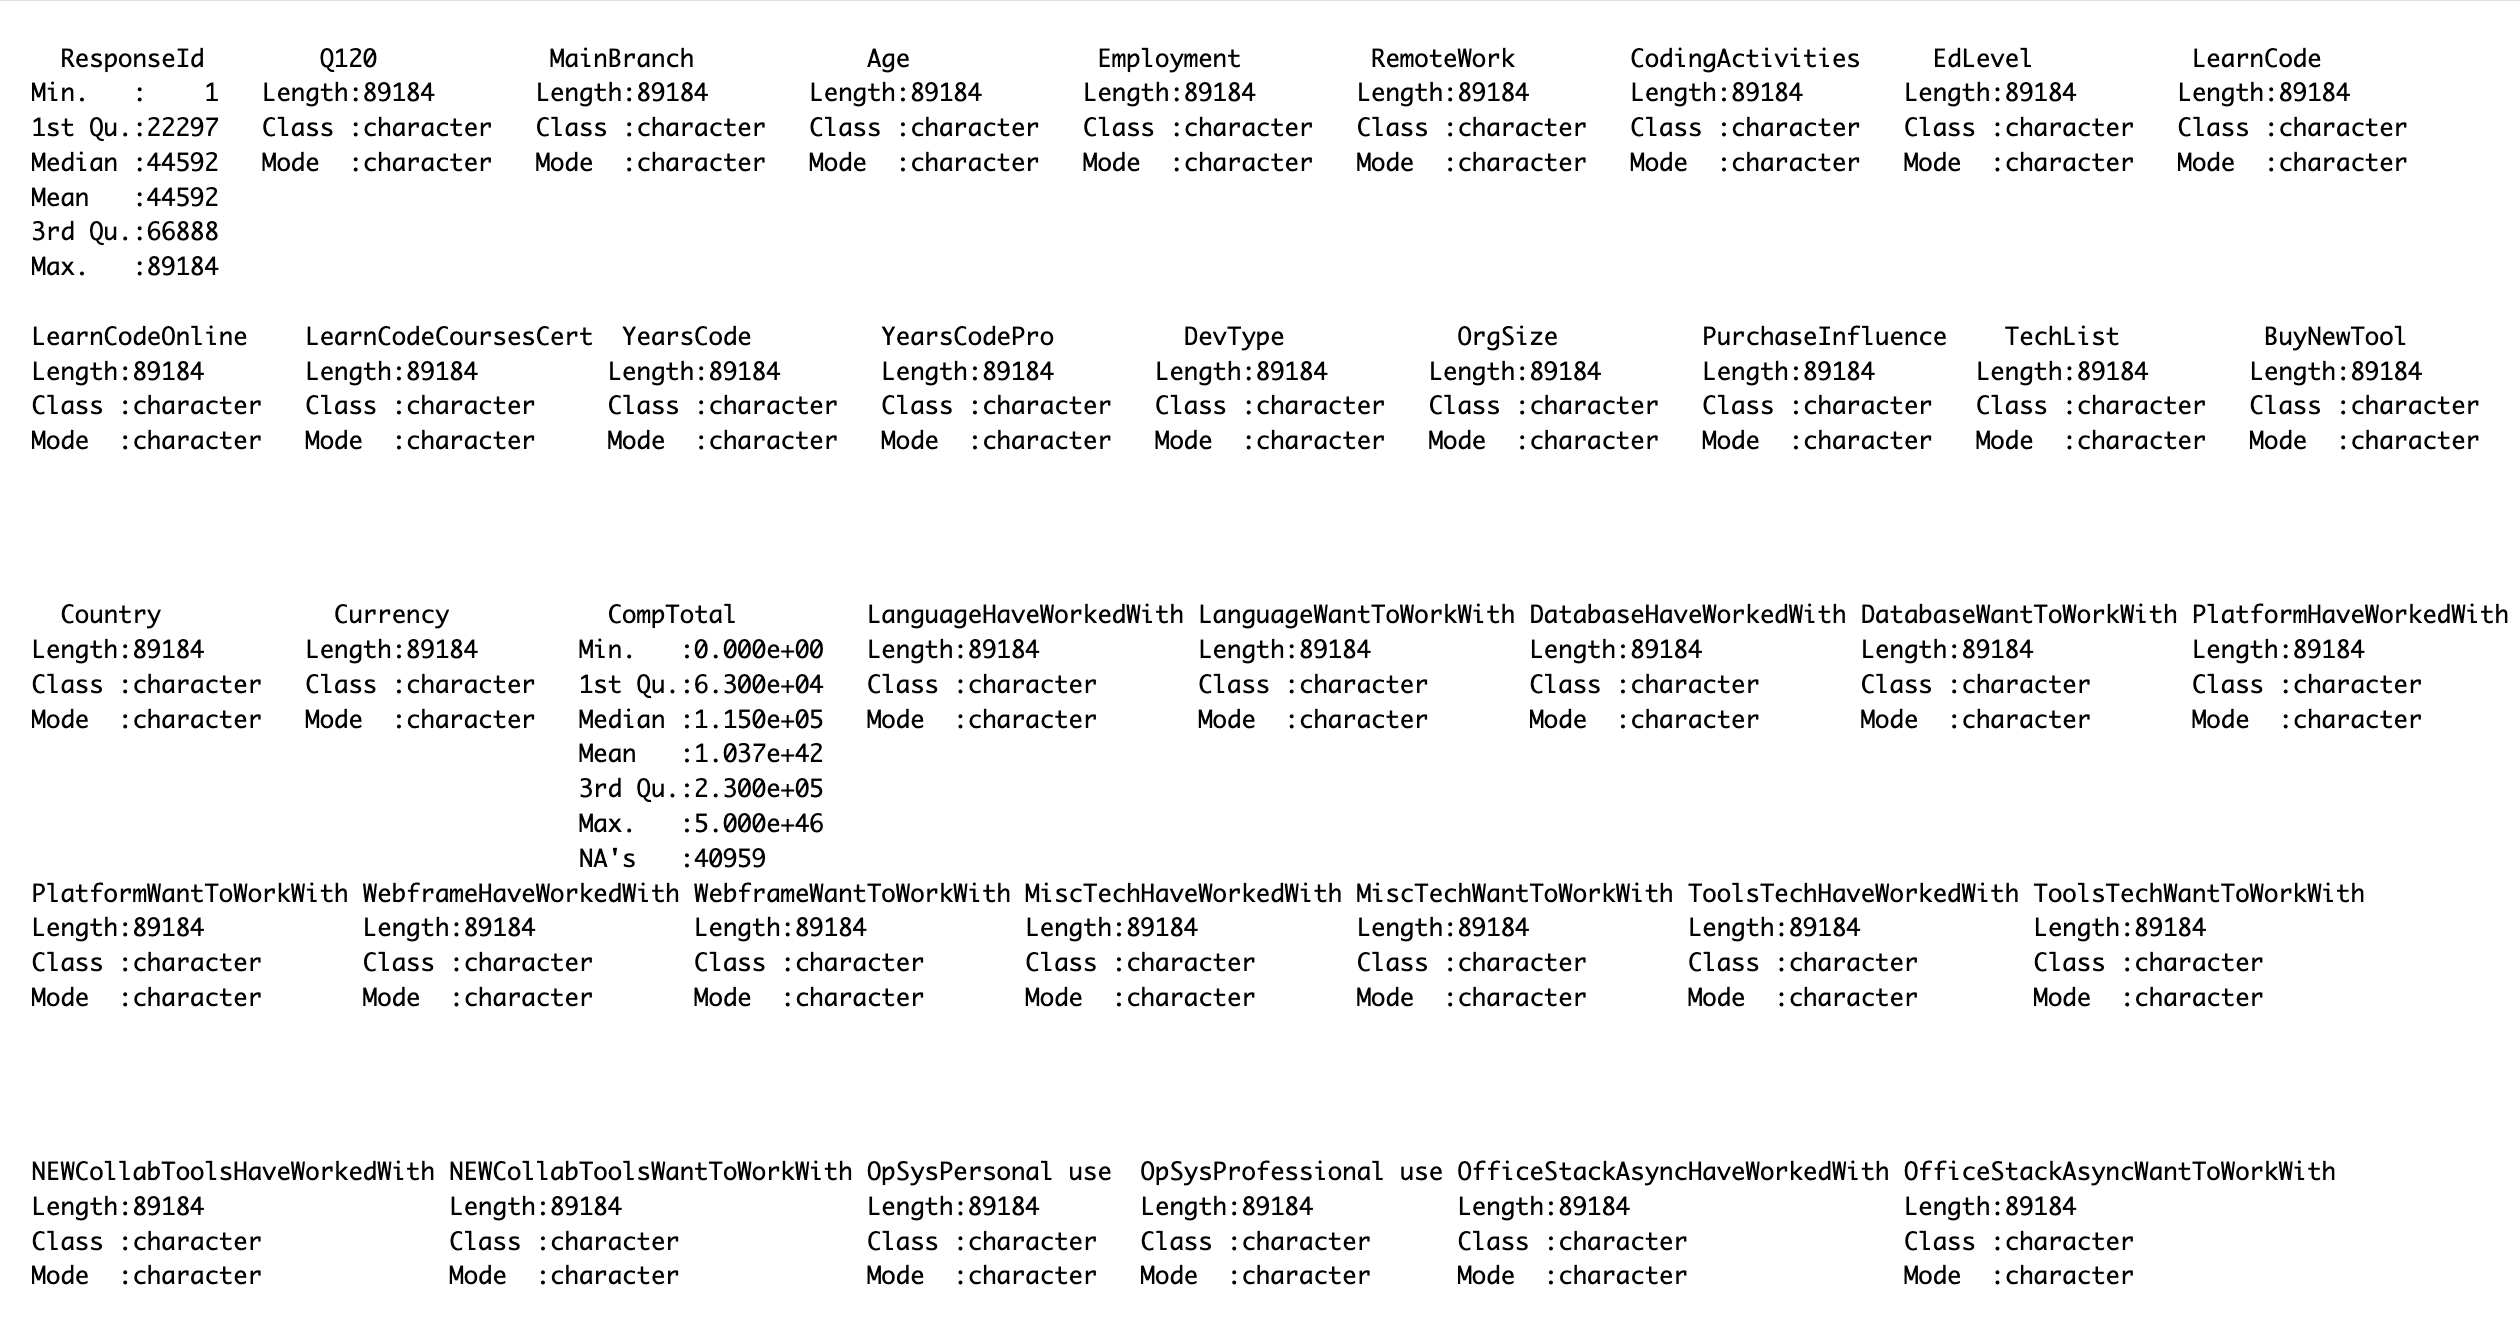
\includegraphics[width=0.5\textwidth,height=0.5\textheight]{Missing_data.png}

\textbf{Numeric Variables} - CompTotal: Extremely right-skewed given
outliers with extremely high compensation values. - ConvertedCompYearly:
Extremely right-skewed given outliers with extremely high compensation
values. - ResponseId: This variable identifies each observation and is
not a response from participants. - WorkExp: Right-skewed, indicating
the decreasing frequency of work experience within the respondants. -
convertedcomp\_log: Given the compensation outliers present within the
dataset, a log transformation has been applied to the variable of
interest `ConvertedCompYearly' resulting in an approximately normal
distribution.

\begin{figure}
\centering
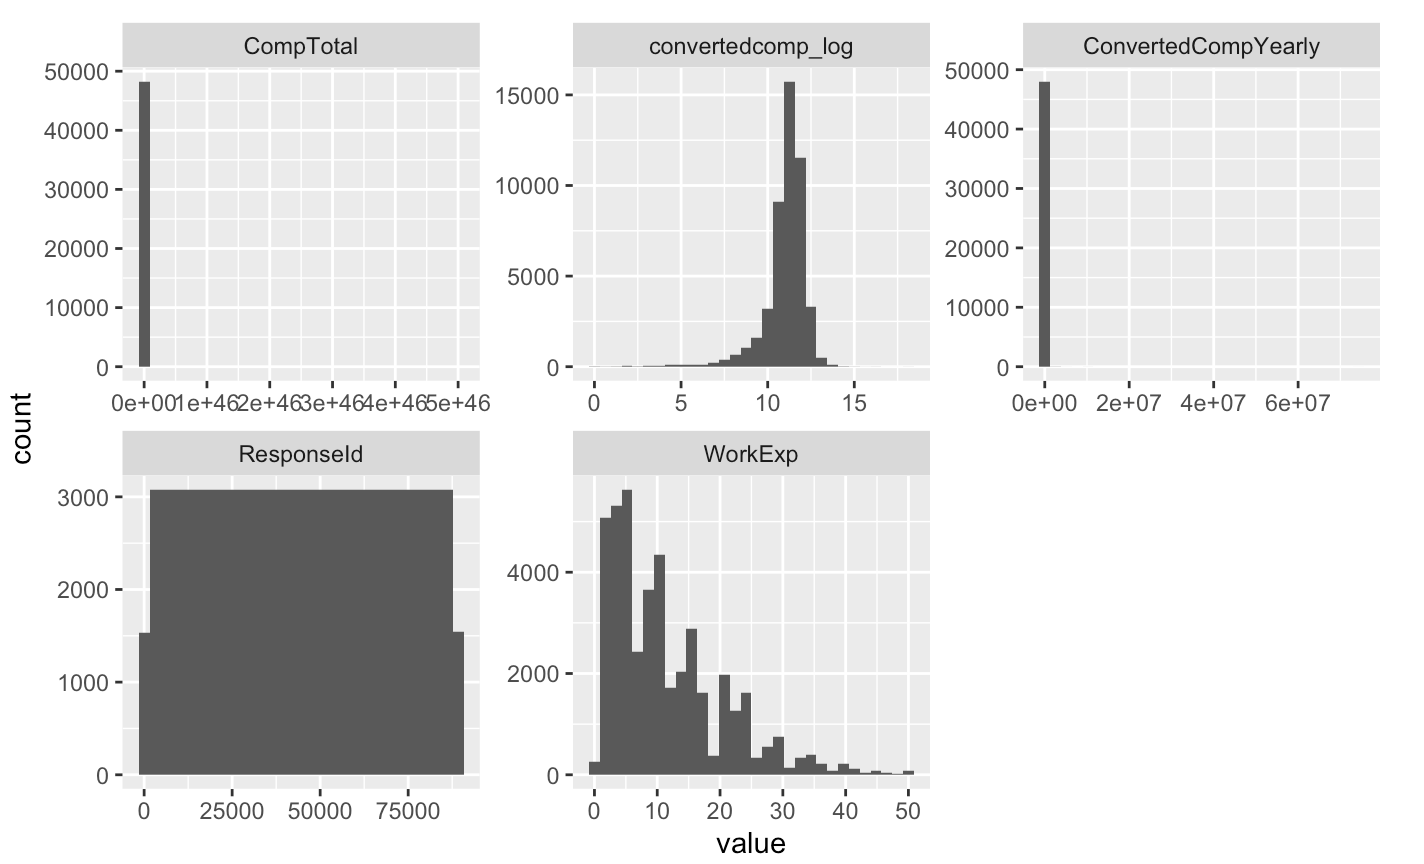
\includegraphics[width=0.5\textwidth,height=0.5\textheight]{Numerical_variables_hist.png}
\caption{Alt text}
\end{figure}

Further visualisation of missing values for key variables of interest: -
There are random missing values across `YearsCode' and `YearsCodePro'. -
Missing values are present across all combinations of `Employment'
types. - A singular `Employment' category has a large number of missing
values, this is the Non-employed category as those without employment
have no compensation. - It is evident that there is a high amount of
non-response questions focused on compensation, with several
`Employment' categories having only missing response variables. This is
on account of the high number of unique `Employment' combinations given
the multi-select string nature of the questions and the sensitivity of
providing compensation information. - No clear trends of missing
variables.

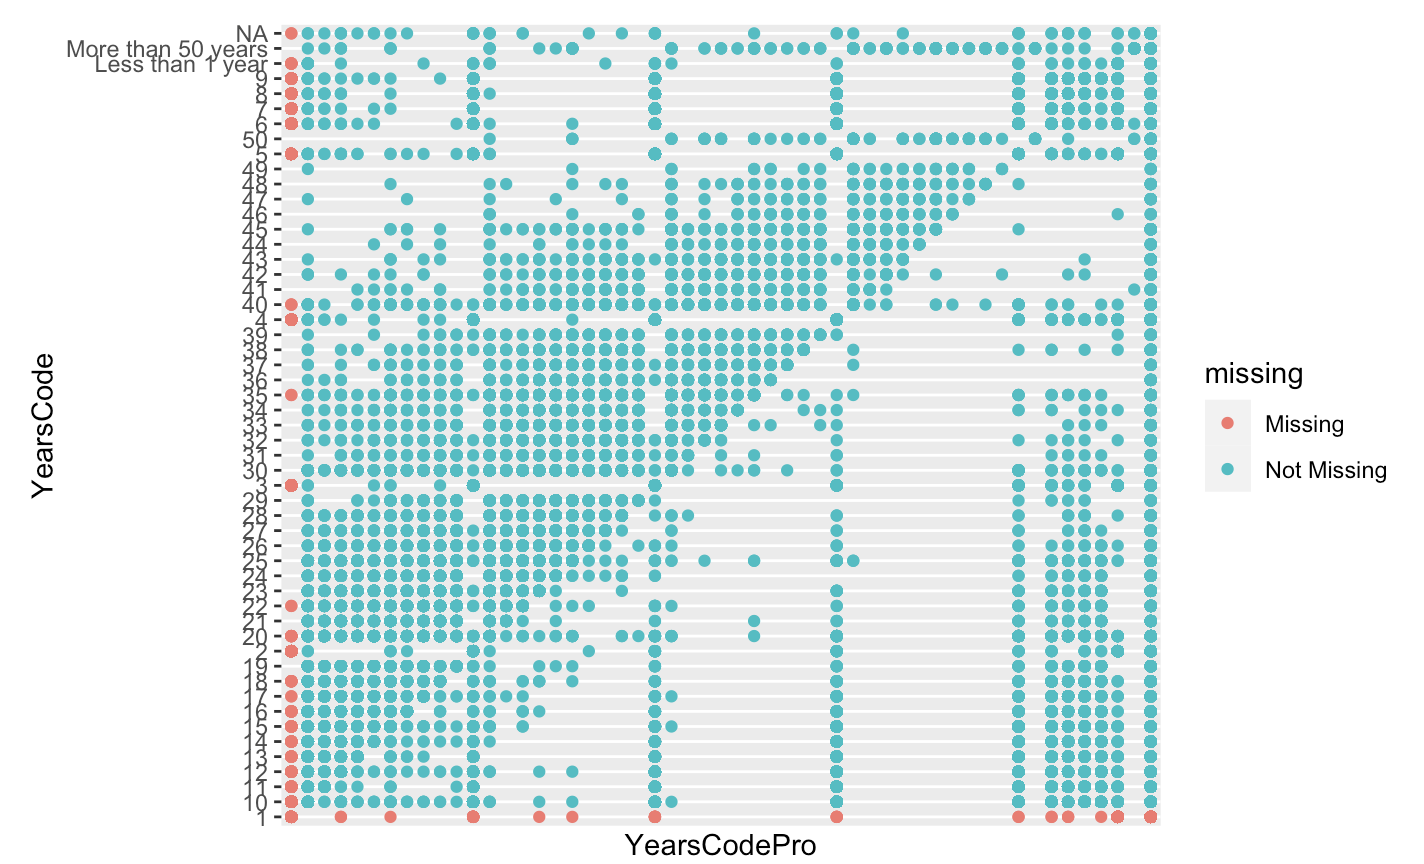
\includegraphics[width=0.5\textwidth,height=0.5\textheight]{MV_YearsCode_vs_Pro.png}
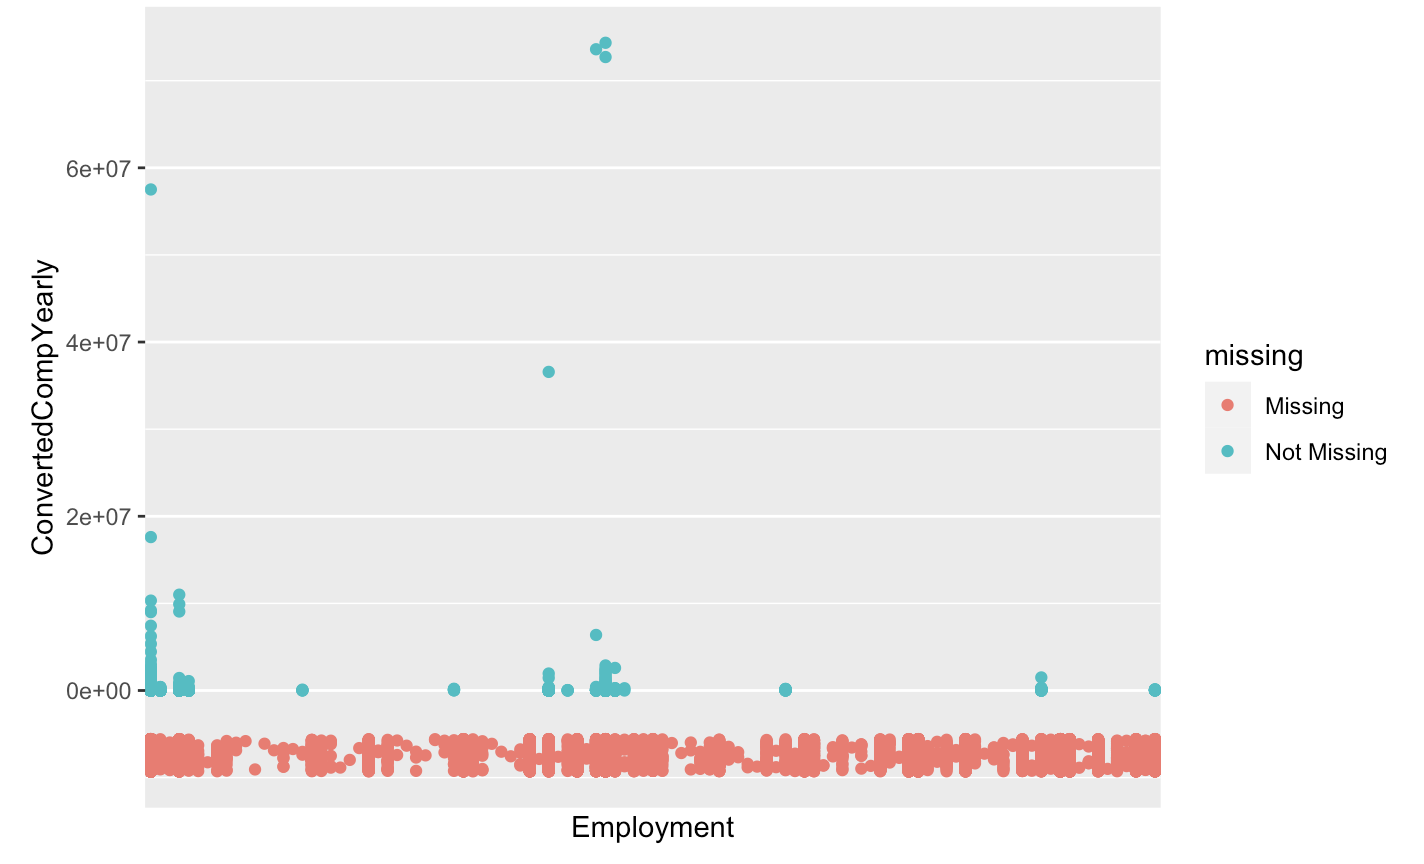
\includegraphics[width=0.5\textwidth,height=0.5\textheight]{MV_Employment_vs_converted_comp.png}

UpSet plots have been used to visualise the intersections of missing
data within our dataset, given several characteristics and attribute
values can be encoded simultaneously (Lex et al, 2014). This plot
indicates that there are higher frequencies for interceptions across a
greater number of variables relating to `AI' and reduced frequencies for
interceptions of various reduced combinations of `AI' attributes. Many
missing values are visibly present within this dataset, therefore
requiring appropriate cleaning methodologies.
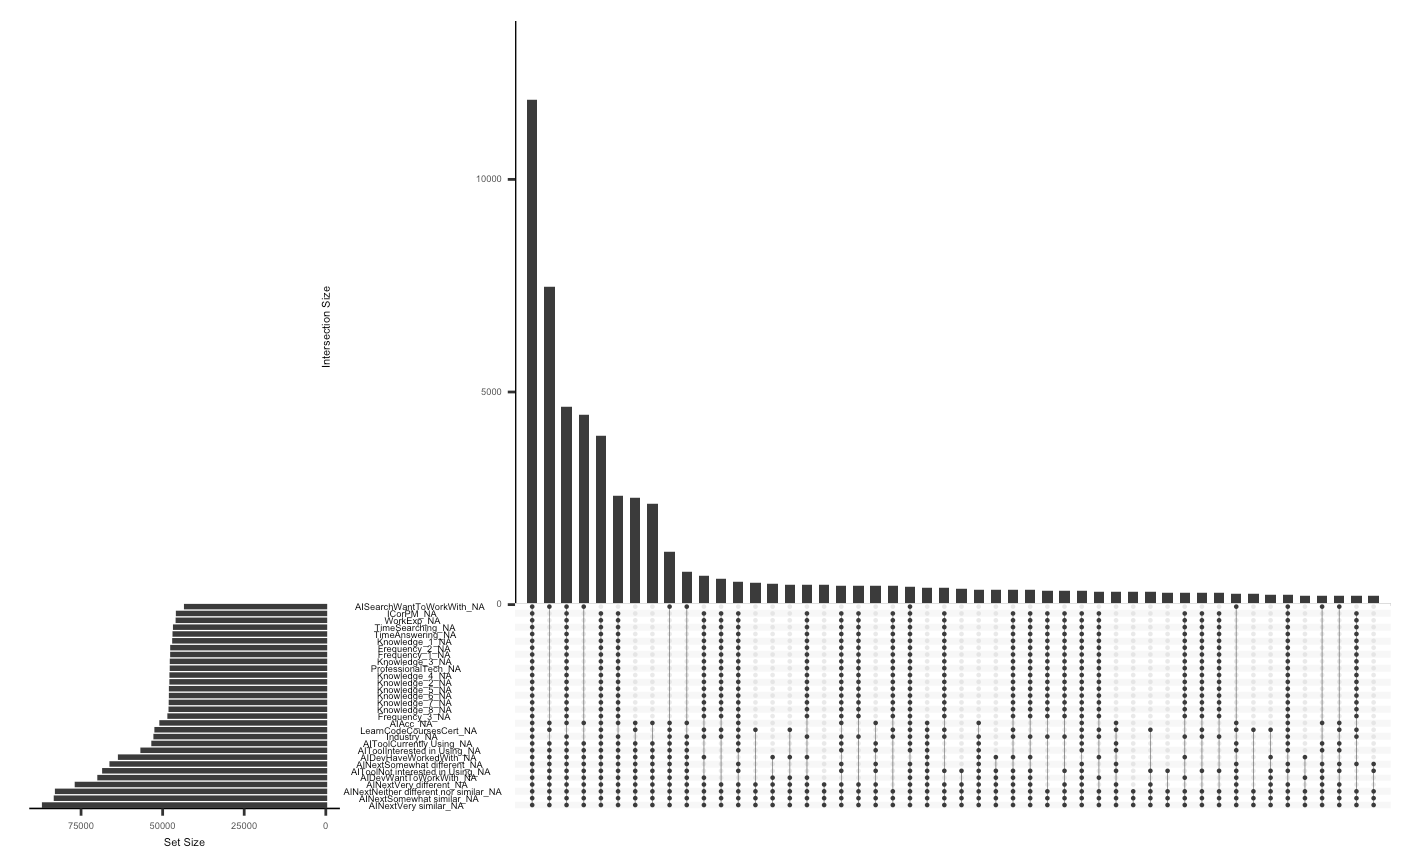
\includegraphics[width=0.5\textwidth,height=0.5\textheight]{Missing_values_upset.png}

\hypertarget{data-cleaning-and-manipulation}{%
\paragraph{Data Cleaning and
Manipulation}\label{data-cleaning-and-manipulation}}

To clean our data, we first began by subsampling the dataset to include
only valid responses to \emph{ConvertedCompYearly}. This decision was
made as it maintains a large dataset (48,019 responses) while ensuring
data integrity. Additionally due to the highly skewed nature of the
data, and \emph{ConvertedCompYearly} being the variable of interest any
self-imputation would have been unreliable.

In order to prepare the data for imputation and subsequent regression
analyses, several variables required augmentation. The
\emph{LanguageHaveWorkedWith} and \emph{DatabaseHaveWorkedWith}
variables contained multiple responses per respondent, indicating every
language or database they had worked with. These variables were
separated and encoded, along with \emph{EdLevel}, \emph{DevType}, and
\emph{OrgSize}, to create binary columns representing each unique
response.

To handle missing values, we employed Multiple Imputation by Chained
Equations (MICE). Five iterations were selected as it gave a balance
between computational efficiency and convergence of the algorithm. For
the encoded binary variables, the logistic regression method (`logreg')
was utilized, for the numeric variable \emph{YearsCode} was imputed
using predictive mean matching (`pmm'), this method preserves the
distributional properties of the original data (van Buuren, 2007).

The MICE algorithm operates by iteratively imputing missing values in
each variable based on the observed values of other variables. By
generating multiple imputed datasets, MICE accounts for the uncertainty
associated with missing data, providing a more robust and reliable basis
for subsequent statistical analyses.

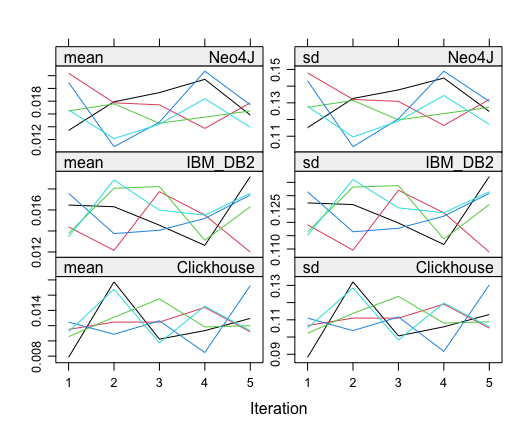
\includegraphics[width=0.5\textwidth,height=0.5\textheight]{wiggle_plots.png}
The plot shows the mean and standard deviation of the imputed values
only. We can see the streams intermingling indicating convergence of the
imputed values.

\hypertarget{feature-selection-and-data-curation}{%
\paragraph{Feature Selection and Data
Curation}\label{feature-selection-and-data-curation}}

In analyzing compensation data problems such as skewness and outliers
are common. These issues can have detrimental effects on the model. To
address this, we performed a log-transformation on the compensation
data. The transformation helped to stabilize variance and normalize the
data, making it suitable for linear modeling.

The transformation's effectiveness is evident in the boxplot comparison
below, which shows a marked reduction in skewness.

\begin{figure}
\centering
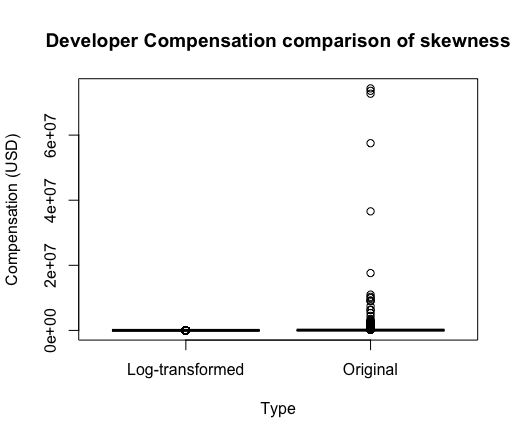
\includegraphics[width=0.5\textwidth,height=0.5\textheight]{comparison_of_skewness.png}
\caption{Alt text}
\end{figure}

To identifying the key determinants of \emph{ConvertedCompYearly}, we
utilized Lasso regression, a regularization method designed to improve
the statistical model's predictive performance and clarity. Lasso
performs both variable selection and regularization, which helps in
handling the multicollinearity and overfitting by shrinking less
important feature's coefficients to zero. Consequently, Lasso enables us
to identify the most pertinent variables while maintaining a
parsimonious model.

Our dataset included 135 features, some of which exhibited high
multicollinearity. Using Lasso regression, we aimed to mitigate these
issues by selecting a subset of features that provides the best
predictive performance.

The cross-validation process for Lasso regression involved tuning the
lambda parameter, which controls the strength of the penalty applied to
features. A plot of the cross-validation results shows how the mean
squared error varies with different log(lambda) values. The optimal
lambda value in this context was approximately -6.502476 in log space.

\begin{figure}
\centering
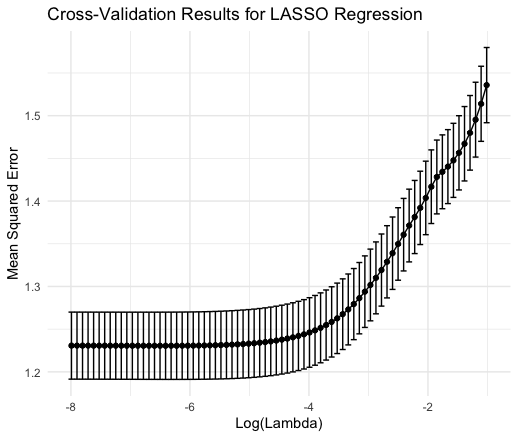
\includegraphics[width=0.5\textwidth,height=0.5\textheight]{cross_validation_results.png}
\caption{Alt text}
\end{figure}

\hypertarget{implimentation}{%
\subsubsection{Implimentation}\label{implimentation}}

All code and algorithms can be viewed via the GitHub repository (see
appendix).

\hypertarget{results}{%
\subsubsection{Results}\label{results}}

\hypertarget{numerical-responses-results}{%
\paragraph{Numerical Response's
Results}\label{numerical-responses-results}}

\begin{itemize}
\tightlist
\item
  The variable chosen for this part was `YearsCode'. Here is the
  histograms:
  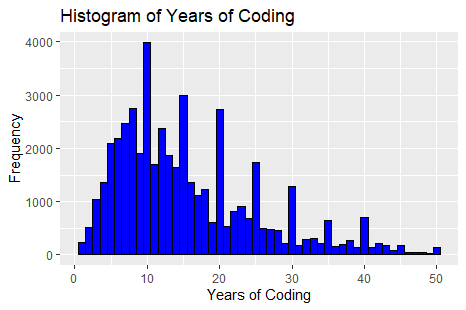
\includegraphics[width=0.8\textwidth,height=0.8\textheight]{yearsCode_numeric_histogram.png}
  There is a noticeable peak in the distribution at 5 to 10 years of
  coding experience, indicating that a high percentage of persons in our
  sample have coding expertise in this area. This might mean that many
  people are in the early to mid stages of their careers. The frequency
  drops as the number of years increases, as is common in many job
  domains where fewer people achieve very high levels of expertise. The
  existence of numerous peaks (10, 15, 20, 30 years) may reflect varied
  common career duration or moments at which people change occupations,
  rise to new roles, or even take pauses from coding. The histogram
  includes a big tail to the right, indicating that there are still a
  considerable number of people with extensive coding expertise, but far
  less than those with 5-10 years. \textbf{Summary Statistics:}
  \textbf{Mean of Years of Coding: 15.67} \textbf{Standard Deviation of
  Years of Coding: 9.87} \textbf{Median of Years of Coding: 13} The
  dataset includes around 15.67 average years of coding experience. The
  mean is sensitive to outliers and skewed distributions, which means
  that a few extremely high or low numbers can have a large impact on
  the mean. A standard deviation of around 9.87 years implies that
  individual coding experience varies greatly from the average (mean),
  with many developers having years of expertise that are significantly
  lower or higher than the norm. The median is a reliable measure of
  central tendency that is less impacted by outliers and skewed data
  than the mean. This number is less than the mean, indicating that the
  distribution of years of coding is somewhat skewed to the right
  (positively skewed), with a tail extending towards greater years of
  coding.
\end{itemize}

\hypertarget{categorical-responses-results}{%
\paragraph{Categorical Response's
Results}\label{categorical-responses-results}}

\begin{itemize}
\tightlist
\item
  Two categorical variable: ``Education Level'' and ``Organisation
  size'' has been chosen to observe if there is any association among
  them. For this hypothesis test, a Fisher Exact Test has been deployed.
  The p-value is derived from a simulation method rather than an exact
  calculation based on 10,000 replicates. This simulation method is
  conducted due to the small expected frequencies in the contingency
  table, making exact calculations impractical. The alternative
  hypothesis of this test is two-sided, indicating that it was examining
  any potential correlation between the variables, without assuming that
  one variable is greater or lesser than the other.
  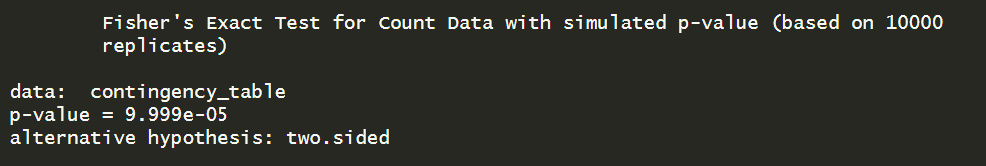
\includegraphics[width=1\textwidth,height=1\textheight]{fisher-test-result.png}
  Using Fisher's Exact Test with 10,000 simulated repetitions, we
  established a very significant connection between the two categorical
  variables under study (p \textless0.0001). This implies that the
  observed link is highly unlikely to have occurred by coincidence,
  providing compelling evidence against the null hypothesis of no
  association. This conclusion might have significant consequences for
  our understanding of education level and organisation size. The
  robustness of this result is reinforced by the use of a simulation
  technique to account for the contingency table's particular
  conditions.
\end{itemize}

\begin{figure}
\centering
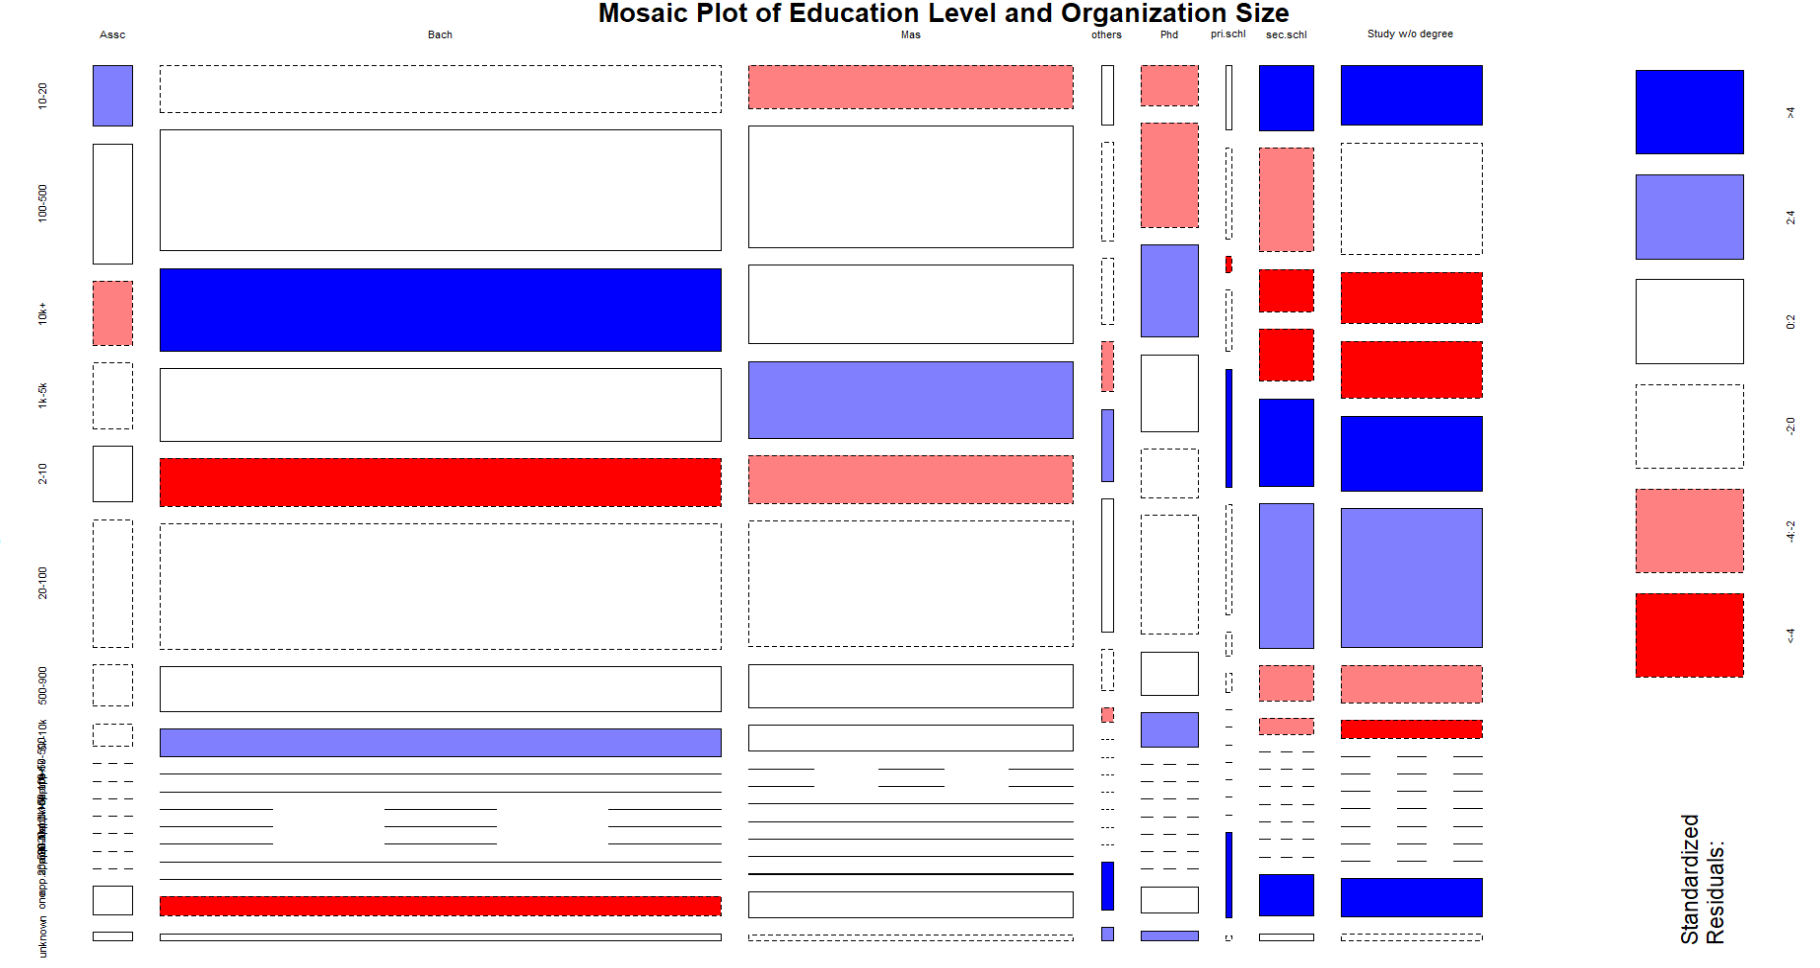
\includegraphics[width=1\textwidth,height=1\textheight]{mosaic-fisher-plot.png}
\caption{Alt text}
\end{figure}

The relationship between organisation sizes and education levels is
comprehensively visualised using the mosaic plot. Different education
levels are represented on the X-axis, and organisational sizes are
represented on the Y-axis. The size of the tiles in the mosaic plot
represents the frequency or proportion of combinations of education
level and organisation size. Each tile represents a combination of these
attributes. The standardised residuals, which show the degree of
association between these categories, are indicated by the colour coding
of the tiles, which ranges from blue to red. Red tiles indicate
lower-than-expected frequencies, and blue tiles indicate
higher-than-expected frequencies. The colour's intensity corresponds to
the size of these residuals.

Several important insights are revealed by a thorough plot analysis. For
developers who possess a bachelor's degree (as shown by the larger blue
tiles), there is a noticeably higher proportion in smaller
organisations. On the other hand, as indicated by the red tiles,
employees with bachelor's degrees tend to be less common than
anticipated in larger organisations. Workers who hold master's degrees
are more common in medium-sized to large-sized businesses; these
positive residuals are highlighted by blue tiles. The red tiles indicate
that employees with master's degrees are less common in smaller
organisations.

In a similar vein, employees with professional degrees are more common
in larger organisations, although the frequency of such employees is
lower in smaller organisations. The trend for developers holding
associate's degrees is less obvious; medium-sized organisations
nevertheless exhibit a somewhat higher frequency than anticipated.

With only slight differences, the proportion of employees who have only
completed their primary or elementary and secondary schooling is
generally low across all organisation sizes. The blue tiles indicate the
higher frequency of employees in smaller organisations who have some
college education but have not earned a degree, while the red tiles
indicate the lower frequency of such employees in larger organisations.

In conclusion, the mosaic plot shows that while smaller organisations
have a more diverse range of education levels, including bachelor's
degrees and some college education without degrees, larger organisations
prefer employees with higher education levels, such as master's and
professional degrees. The standardised residuals provide important
information about the hiring practices of various organisation sizes by
highlighting the significant relationships between education levels and
organisation sizes

\hypertarget{regression-results}{%
\paragraph{Regression Results}\label{regression-results}}

\begin{figure}
\centering
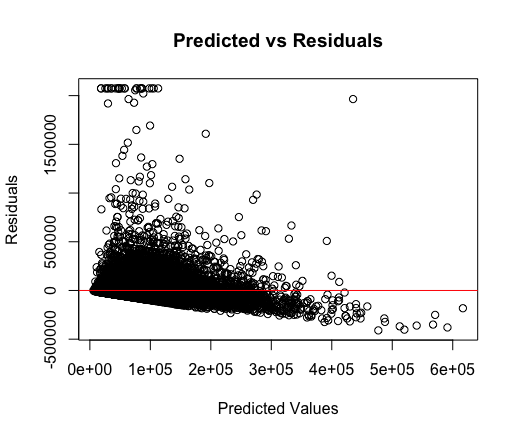
\includegraphics[width=0.5\textwidth,height=0.5\textheight]{predicted_vs_residuals.png}
\caption{Alt text}
\end{figure}

The Predicted vs Residuals plot displays residuals on the vertical axis
and the predicted compensation values on the horizontal axis. A
horizontal line at zero represents no error between the predicted and
actual values. The ideal scenario in such a plot is for the residuals to
be randomly dispersed around the horizontal line, indicating that the
model predicts equally well across all values of the independent
variable. As can be observed, the spread of residuals increases with the
predicted compensation values. The heteroscedasticity observed suggests
that the model's predictive accuracy varies across the scale of
compensation, being less precise at higher compensation levels. This
violates one of the fundamental assumptions of linear regression, so
further results should be treated with caution.

\textbf{Model Performance}

The Mean Squared Error of the model was found to be approximately
464,518,156,488. This high value suggests that the model may have
limitations in capturing all the variability in the compensation data.
The R-squared value was -0.0004, indicating that the model explains none
of the variability around the mean. This unexpectedly low value could be
a result of non-linear relationships not captured by the model.

The top predictors determined by the Lasso of developer compensation
include:

\textless\textless\textless\textless\textless\textless\textless{} HEAD -
Student: Coefficient: -1.15, 95\% CI: {[}-1.30, -1.00{]}. Suggests that
attaining education can have a negative impact on compensation. - APL:
Coefficient: -0.53, 95\% CI: {[}-0.65, -0.41{]}. Suggests that less
mainstream technologies may correlate with lower pay. - Academic
Researcher: Coefficient: -0.31, 95\% CI: {[}-0.42, -0.196{]}. Indicates
lower compensation in academic roles. - Primary/Elementary School:
Coefficient: -0.17, 95\% CI: {[}-0.336, 0.0{]}. Suggests lower
compensation for lower educational attainment. - Senior Executive
(C-Suite, VP, etc.): Coefficient: 0.28, 95\% CI: {[}0.194, 0.368{]}.
Senior positions result in higher compensation. ======= - Student:
Coefficient: -1.15, 95\% CI: {[}-1.30, -1.00{]}. This indicates that
being a student is associated with lower compensation, possibly due to
part-time or intern-level employment. - APL: Coefficient: -0.53, 95\%
CI: {[}-0.65, -0.41{]}. Suggests less mainstream technologies may
correlate with lower pay. - Academic Researcher: Coefficient: -0.31,
95\% CI: {[}-0.42, -0.196{]}. Indicating lower compensation in academic
roles. - Primary/Elementary School: Coefficient: -0.17, 95\% CI:
{[}-0.336, 0.0{]}. Suggests lower compensation for lower educational
attainment. - Senior Executive (C-Suite, VP, etc.): Coefficient 0.28,
95\% CI: {[}0.194, 0.368{]}. Senior positions result in higher
compensation.

\begin{itemize}
\tightlist
\item
  Raku: Coefficient: -0.37, 95\% CI: {[}-0.49, -0.25{]}. Similar to APL,
  using less common technologies correlates with lower compensation.
\item
  Company size showed that large companies compensate better than small
  companies, with large companies having a positive coefficient
  (Coefficient: 0.34, 95\% CI: {[}0.294, 0.381{]}) and small companies a
  negative coefficient (Coefficient: -0.32, 95\% CI: {[}-0.367,
  -0.263{]}).
\item
  Blockchain (Coefficient: 0.05, 95\% CI: {[}0.0, 0.1{]}) and Snowflake
  (Coefficient: 0.31, 95\% CI: {[}0.263, 0.357{]}): These technologies
  are associated with higher compensation, likely reflecting their
  current demand and the specialization required.
\end{itemize}

The Lasso model has provided valuable insights into the factors
affecting developer compensation, highlighting the role of job roles,
technology use, and company size. However, the low R-squared value
suggests that additional variables, possibly capturing more specific
skills or regional economic factors, might be needed to improve the
model's explanatory power. Further analysis could also explore
non-linear modeling techniques or more sophisticated transformations to
better capture the complex dynamics of the compensation landscape in
tech.

\hypertarget{discussion}{%
\subsubsection{Discussion}\label{discussion}}

\hypertarget{successes}{%
\paragraph{Successes}\label{successes}}

The data for the analysis we conducted was challenging to process due to
a significant amount of missing values. Our most significant success was
using the Multiple Imputation with Chained Equations (MICE) algorithm to
handle missing values, which we did satisfactorily. By using five
iterations, we ensured that our data was balanced. Successful
implementation of the MICE algorithm ensured that the imputed data sets
were reliable and robust, providing a solid foundation for subsequent
analysis. So, we encountered convergence issues in our data and ensured
that model parameters were stable and gave accurate and reliable
results.

In addition, we effectively handled the data cleaning and manipulation
process. Due to the highly skewed structure of the
\emph{ConvertedCompYearly} variable, which we chose as the response
variable, performing an analysis in its raw form would not allow us to
obtain accurate results. Maintaining a large dataset of 48,019 responses
while ensuring data integrity, we began \emph{ConvertedCompYearly} by
subsampling the dataset to include only valid responses. Through this
careful data preparation and the application of statistical methods
detailed above, we successfully prepared the data for accurate and
meaningful analysis.

\hypertarget{limitations}{%
\paragraph{Limitations}\label{limitations}}

Although the research is comprehensive and informative, it also comes
with some limitations that should be considered when interpreting the
results. Firstly, the survey is not fully randomized; it mostly targets
users who are active on Stack Overflow. This method of surveying through
Stack Overflow's own channels, such as onsite messaging, blog posts, and
emails, can be limiting. Additionally, only two rounds of survey sending
may include a limited variety of respondents.

Another important consideration is that the salary question was
optional, and 48,026 respondents provided salary data. This means that
nearly half of the participants chose not to give this information.
Different factors can lead to this, such as the sensitivity of salary
data in some countries and cultures, or individuals not feeling
comfortable sharing their earnings, especially if they are dissatisfied
with them.

Data privacy and security are also critical concerns. Due to worries
about declaring sensitive information, participants may hesitate to
share detailed personal data. The sensitivity of the information, the
people who have or can access the information, and the security
solutions can be concepts that stop people. In today's digital world,
concerns about personal information breaches can significantly affect
participation rates.

To ensure data consistency, salary data provided by the participant was
converted to US dollars using the exchange rate on June 2, 2023.
However, this conversion may lead to biases. Economic conditions can
differ between countries, so an individual earning a good salary by
their country's standards might fall into a different income category
after conversion to USD. This could lead to incorrect findings when
making country-based inferences.

\hypertarget{conclusion}{%
\subsubsection{Conclusion}\label{conclusion}}

The Stack Overflow Annual Developer Survey 2023 is a noteworthy dataset
that offers valuable insights into developer compensation trends and
their factors.

Our results indicate that not only does education and company size
impact compensation but specific technologies that are both widely used,
and in-demand drive increased compensation values. This is in alignment
with the economic theory of supply and demand, in which compensation
increases when there is a greater amount of demand to supply. To obtain
more accurate results, further analysis is required with a higher degree
of granularity for elements related to compensation and the possible
application of non-linear models. Considering that many survey items
were optional, this will lead to a deeper comprehension of the effects
on compensation.

The Stack Overflow Developer Survey for 2023 has provided valuable
insights into understanding compensation of developers across the world.
This report has addressed a number of data challenges including the
non-response to identify the relationships of key variables that impact
developer compensation. Further research may deepen our understanding of
factors that may influence the future of developers as they grow, learn
and adjust to new trends and technologies in the rapidly evolving
industry. This analysis does not only benefit developers but may be used
by employers and policymakers to improve their understanding of the
compensation landscape for developers and address disparities across the
industry.

\hypertarget{references}{%
\subsubsection{References}\label{references}}

Corry, N.H., Williams, C.S., Battaglia, M., McMaster, H.S., Stander,
V.A., (2017), Assessing and adjusting for non-response in the Millennium
Cohort Family Study. \emph{BMC Med Res Methodol}, 17(16).
\url{https://doi.org/10.1186/s12874-017-0294-8} \newline Heeringa, S.
G., West, B. T., \& Berglund, P. A. (2017). Applied Survey Data Analysis
(2nd ed.) \newline Kelly K, CLARK B, Brown V,Sitzia J. (2003). Good
practice in the conduct and reporting of survey research,
\emph{International Journal for Quality in Health Care}, 15(3),
261--266, \url{https://doi.org/10.1093/intqhc/mzg031} \newline Lex, A.,
Gehlenborg, N., Strobelt, H., Vuillemot, R., \& Pfister, H.
(1983--1992). UpSet: Visualization of Intersecting Sets. \emph{IEEE
transactions on visualization and computer graphics}, 20(12),
\url{https://doi.org/10.1109/TVCG.2014.2346248} \newline Pickery, J., \&
Carton, A. (2008). Oversampling in Relation to Differential Regional
Response Rates. \emph{Survey Research Methods}, 2(2), 83--92.
\url{https://doi.org/10.18148/srm/2008.v2i2.656} \newline van Buuren S.
(2007). Multiple imputation of discrete and continuous data by fully
conditional specification. \emph{Statistical methods in medical
research}, 16(3), 219--242.
\url{https://doi.org/10.1177/0962280206074463}

\hypertarget{appendix}{%
\subsubsection{Appendix}\label{appendix}}

Link to repository:
(\url{https://github.com/JohnBenson-macq/STAT8101_Group_Assignment})

\end{document}
